\documentclass[11pt,a4paper]{article}

%francais
\usepackage[utf8]{inputenc}   
\usepackage[T1]{fontenc}           
\usepackage[francais]{babel}  

%2col/présentation de la page
\usepackage[hmarginratio=1:1,margin=20mm,columnsep=20pt]{geometry}
       
%images
\usepackage{float}
\usepackage{graphicx}
\usepackage{caption}
\addto\captionsfrench{\renewcommand{\figurename}{\textsc{Image}}}

%liens
\usepackage{hyperref}
\hypersetup{breaklinks=true}
\urlstyle{same}

%joli
\usepackage{enumerate}
\usepackage{enumitem}
\setitemize{label=$\bullet$}%,leftmargin=*,topsep=0pt,noitemsep,parsep=0pt}
\usepackage{amsmath,amssymb,amsfonts}
\usepackage{xcolor}
\usepackage[lighttt]{lmodern}

%tableaux
\usepackage{makecell}
\renewcommand\theadalign{cb}
\renewcommand\theadfont{\bfseries}
\renewcommand\theadgape{\Gape[4pt]}
\renewcommand\cellgape{\Gape[4pt]}

%schémas
\usepackage{tikz}
\usetikzlibrary{positioning}

%subdivisions
\usepackage{titlesec}
%\titleformat{\section}{\normalfont\bfseries}{}{1pt}{\normalfont\bfseries}{}
%subsubsub section
\usepackage{titlesec}

%code
\usepackage{listings}
\usepackage{adjustbox}

%algo
\usepackage[]{algorithm2e}

%environnement
\newenvironment{code}{
\footnotesize%
\ttfamily%
\begin{adjustwidth}{2.2em}{0em}%
}
{%
\end{adjustwidth}%
\normalfont%
\normalsize%
}

%en-têtes
\usepackage{fancyhdr}
% style première page
\fancypagestyle{plain}{%
  \fancyhf{}%
\fancyfoot[C]{\thepage}
% Line at the header invisible
  \renewcommand{\headrulewidth}{0pt}
}
%style autres pages
\pagestyle{fancy}%
  \fancyhf{}%

%subsubsubsection command
\setcounter{secnumdepth}{4}
\setcounter{tocdepth}{4}

%formatage des titres de paragraphes comme subsubsubsection
\titleformat{\paragraph}
{\normalfont\normalsize\bfseries}{\theparagraph}{1em}{}
\titlespacing*{\paragraph}
{0pt}{3.25ex plus 1ex minus .2ex}{1.5ex plus .2ex}


%%%%%%%%%%%% :TODO: : noms
\fancyhead[R]{\textsc{Couvreur} Alexis}
%%%%%%%%%%%% :TODO: : titre
\fancyhead[L]{\textsc{Évaluation de différents algorithmes de calcul des composantes fortement connexes}}
\fancyfoot[C]{\thepage}%


\setlength\parindent{9pt}
\pagenumbering{arabic}

\begin{document}


\pagestyle{empty}

\begin{center}
{\LARGE Théorie des Graphes} \\[.8cm]
{\LARGE Évaluation de différents algorithmes de calcul des composantes fortement connexes} \\[.8cm]
{\large \textsc{Couvreur} Alexis \quad} \\[2cm]
\end{center}

\tableofcontents


\clearpage

\pagestyle{fancy}

\section{Description de l'environnement}
Le programme d'évaluation a été fait sous Java 1.8, il nécessite une augmentation de la taille de la pile pour fonctionner ($-Xss4m$). Un processeur IntelCore i7 4 cœurs physiques à 4.3 GHz chacun , mais comme le programme n'est pas parallélisé, le nombre de cœurs importe peu.

\section{Description de l'implémentation des différents modèles de données}
Les graphes sont des graphes orientés à matrice d'adjacence de taille \textit{V*V}.\linebreak
Le nombre de nœuds et d'arcs est gardé en mémoire respectivement dans les variables \textit{V} et \textit{E}.\linebreak
Tous les nœuds et arcs sont donc déduits de la matrice d'adjacence et aucune classe n'a été créée pour les représenter, il s'agit seulement d'entiers tel que $\forall_v, v \in [0, V[$.\linebreak
Ainsi on a comme coût :
\begin{itemize}
\item Est-ce que \textit{i} et \textit{j} sont reliés? : $\mathcal{O}(V)$
\item Combien \textit{i} a-t-il de voisins? : $\mathcal{O}(V)$
\item Quels sont les voisins de \textit{i}? : $\mathcal{O}(V²)$
\item Ajouter l'arc \textit{(a,b)} : $\mathcal{O}(1)$ 
\item Supprimer l'arc \textit{(a,b)} : $\mathcal{O}(1)$ 
\item Combien y a-t-il de nœuds? : $\mathcal{O}(1)$
\item Combien y a-t-il d'arcs? : $\mathcal{O}(1)$
\end{itemize}
Ce qui nous intéresse le plus ici est donc de pouvoir ajouter ou supprimer des arcs, car pour évaluer les algorithmes, on va augmenter le nombre d'arcs uniquement pour un cas de test. On augmentera la taille du graphe (son nombre de nœuds) pour comparer l'effet de la taille du graphe sur les algorithmes.\linebreak


\pagebreak
\section{Description de l'implémentation des différents algorithmes}

\subsection{Algorithmes de calcul de composantes fortement connexes}
Les algorithmes sont généralisés à travers une interface \textbf{SCC} et implémentent  les méthodes :
\begin{itemize}
\item \textit{boolean isStronglyConnected(int v, int w)} : renvoie vrai si \textit{v} et  \textit{w} sont dans la même composante fortement connexe, renvoie faux sinon.
\item \textit{int getCount()} : renvoie le nombre de composantes fortement connexes.
\item \textit{int id(int v)} : renvoie l'id de la composante fortement connexe.
\end{itemize}

\subsection{Algorithme de Tarjan}

\subsubsection{Complexité}
La complexité de l'algorithme de Tarjan est de $\mathcal{O}(|V|+|E|)$.

\subsubsection{Implémentation}
Implémenté en suivant le pseudo code du cours :
\begin{itemize}
\item Une \textit{pile P}
\item Un \textit{tableau booléen dans\_P} de taille \textit{V}, cela évite de faire appel à la méthode \textit{contains} de \textit{Stack} qui est en $\mathcal{O}(N)$ tandis que le tableau est en $\mathcal{O}(1)$
\item Chaque sommet a des propriétés : son numéro, et son numéro accessible
\item Une partition représentant les différentes CFC.
\end{itemize}

\subsubsection{Appréciation}
L'algorithme de Tarjan n'est pas instinctif mais n'est pas très compliqué à comprendre, ce qui rend son implémentation plus simple et agréable.

\subsection{Algorithme de Kosaraju}

\subsubsection{Complexité}
La complexité de l'algorithme de Kosaraju est de $\mathcal{O}(|V|+|E|)$.

\subsubsection{Implémentation}
Implémenté en suivant le pseudo code du cours :
\begin{itemize}
\item Une \textit{pile S} : les sommets visités depuis un sommet v au travers d'une dfs dans le reverse graphe
\item Un \textit{tableau booléen visited} de taille \textit{V}, qui permet de savoir si un sommet a été visité
\end{itemize}


\subsubsection{Appréciation}
L'algorithme de Kosaraju est simple à comprendre, il est très élégant car on utilise l'inverse du graphe, ce qui lui coûte beaucoup en performance.

\pagebreak
\subsection{Algorithme de Gabow}

\subsubsection{Complexité}
La complexité de l'algorithme de Gabow est de $\mathcal{O}(|V|^3)$.

\subsubsection{Implémentation}
Implémenté en suivant le pseudo code du cours :
\begin{itemize}
\item Une \textit{pile S} : pile des sommets non affectés à une CFC
\item Une \textit{pile P} : pile des sommets dont on ne sait pas si ils appartiennent à une CFC différentes de celles trouvées
\item Chaque sommet a son numéro (tableau I dans le code, il contiendra à la fin l'id de la CFC)
\end{itemize}

\subsubsection{Appréciation}
L'algorithme de Gabow n'est pas évident à comprendre et difficile à mettre en œuvre, mais est relativement très puissant.

\pagebreak
\section{Évaluation des différents algorithmes}

\subsection{Jeu de données}

Un graphe $G$ avec $V$=\{5000, 10000, 25000\} et $E$=0 en premier lieu.\linebreak
Nous cherchons à évaluer le temps de calcul des composantes fortement connexes en fonction de la densité du graphe $G$. On suppose que plus le graphe sera dense, plus le temps de calcul sera élevé.
Pour évaluer nous allons effectuer $X$ itérations dans lesquelles nous allons augmenter le nombre d'arcs tel que

\begin{algorithm}
\KwData{Integer X : nombre d'itérations, DirectedGraph G}
\For{$i \in X$}{
	
	$sauvegarderTemps(Tarjan(G))$\;
	$sauvegarderTemps(Kosaraju(G))$\;
	$sauvegarderTemps(Gabow(G))$\;
	
	pour chaque arc de G
	\For{$v \in G.V$}{
		ajouter $X$ arcs\;
		\For{$x \in X$}{
			ajouter un arc entre $v$ et $x*i$ dans $G$\;
		}
	}
}
\end{algorithm}

ce qui nous donne une densité de graphe allant de 0 (à la première itération) à 1 (à la dernière itération) et donc  de $V$ composantes fortement connexes à 1.

Voici le nombre de composantes fortement connexes en fonction de la densité : 

\begin{center}
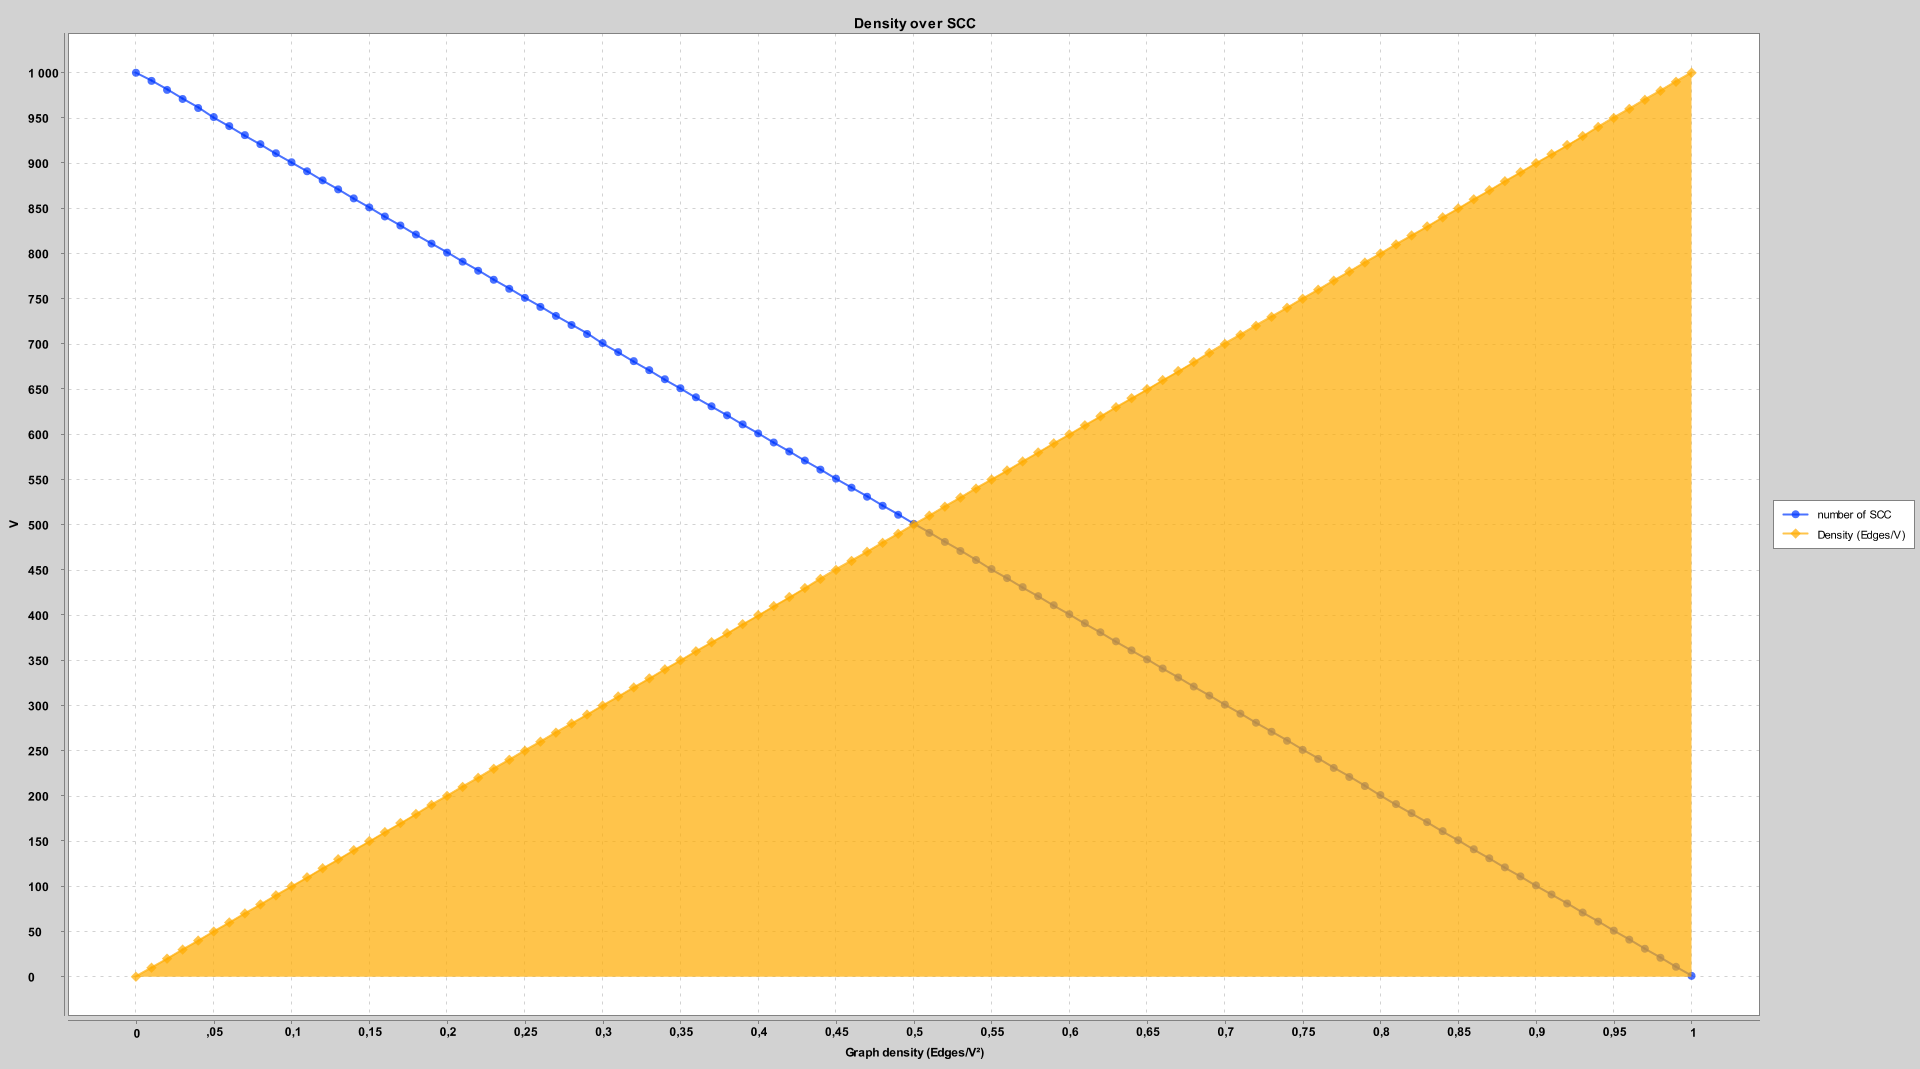
\includegraphics[keepaspectratio=true,width=\linewidth]{./Density-SCC.png}
\captionof{figure}{Rapport entre le nombre de CFC dans le graphes et la densité du graphe}
\end{center}

\pagebreak
\subsection{Résultats}

\subsubsection{V=5000}
\textbf{Soit un total de \underline{25 000 000} d'arcs lorsque la densité vaut 1.}
\begin{center}
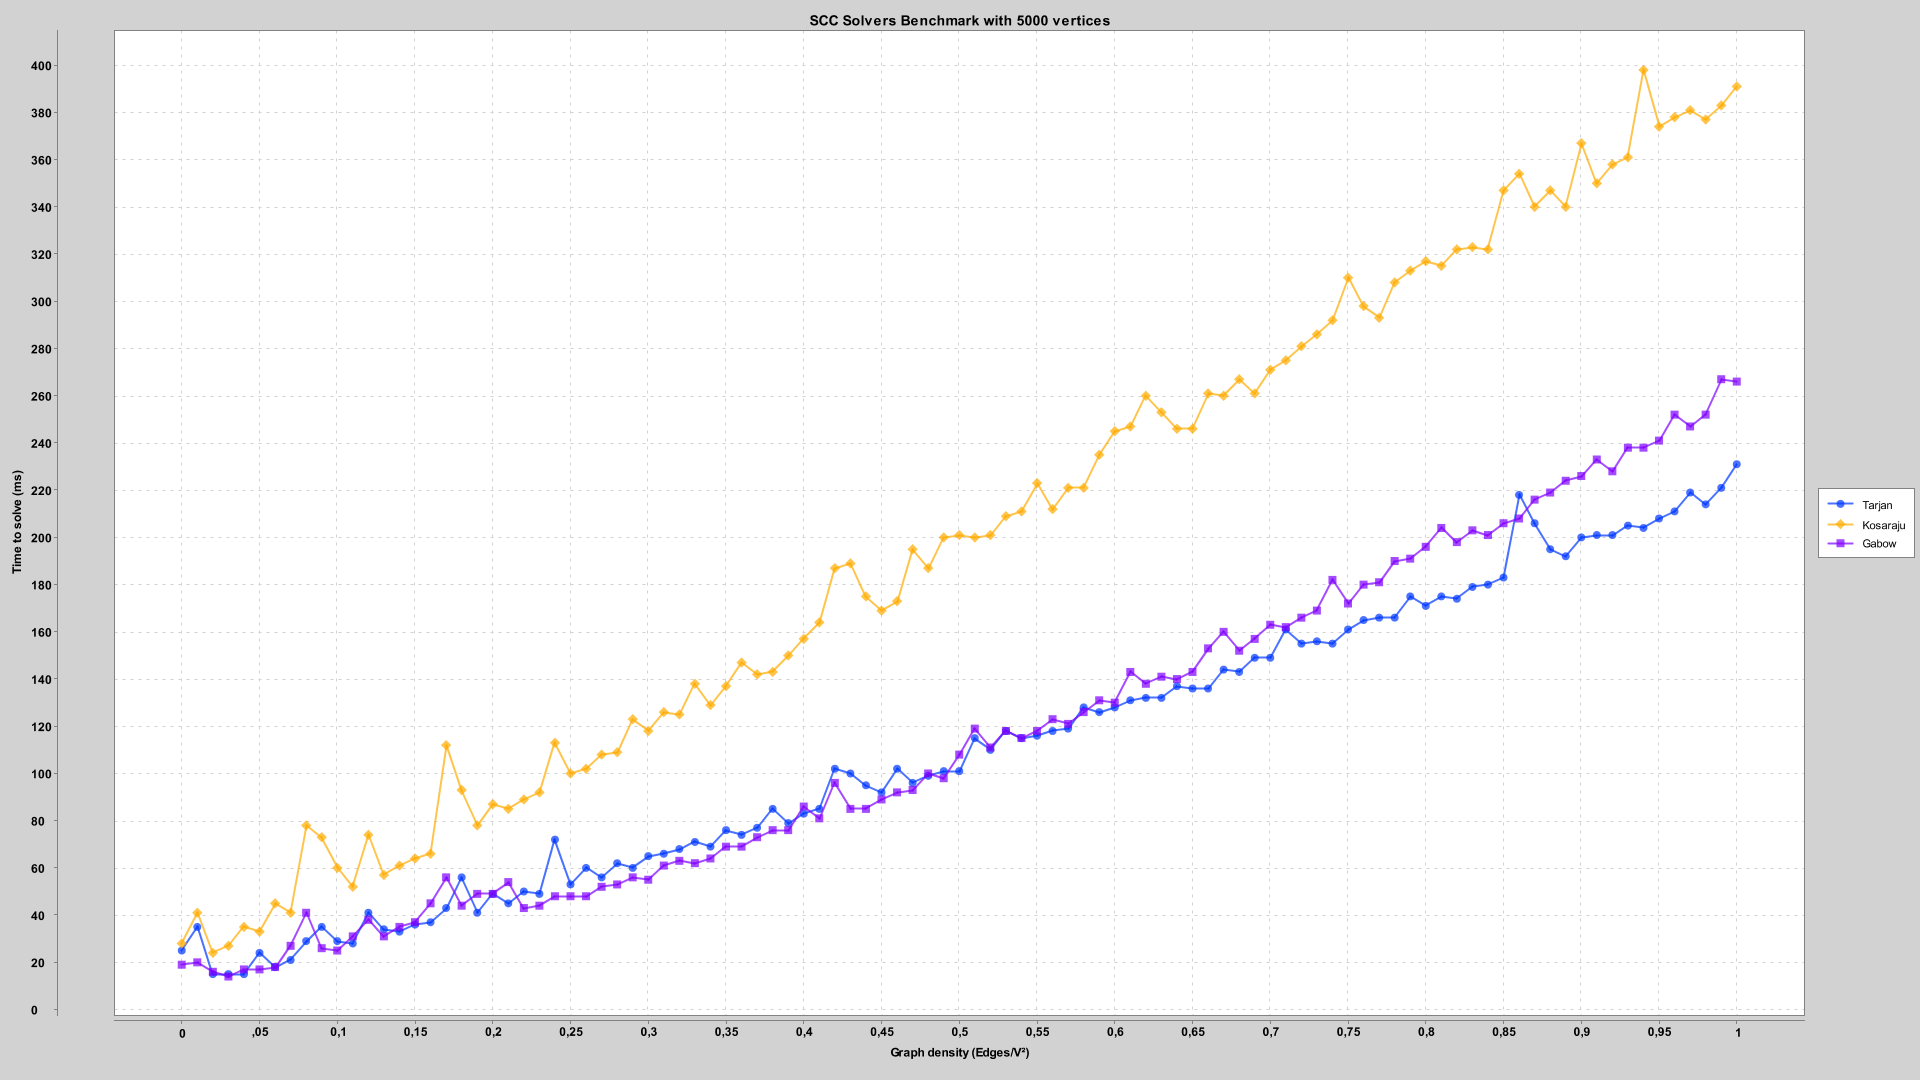
\includegraphics[keepaspectratio=true,width=\linewidth]{./SCCSolvers_5000.png}
\captionof{figure}{Évaluation de différents algorithmes de calcul de composantes fortement connexes en fonction de la densité d'un graphe à 5000 nœuds}
\end{center}

\subsubsection{V=10000}
\textbf{Soit un total de \underline{100 000 000} d'arcs lorsque la densité vaut 1.}
\begin{center}
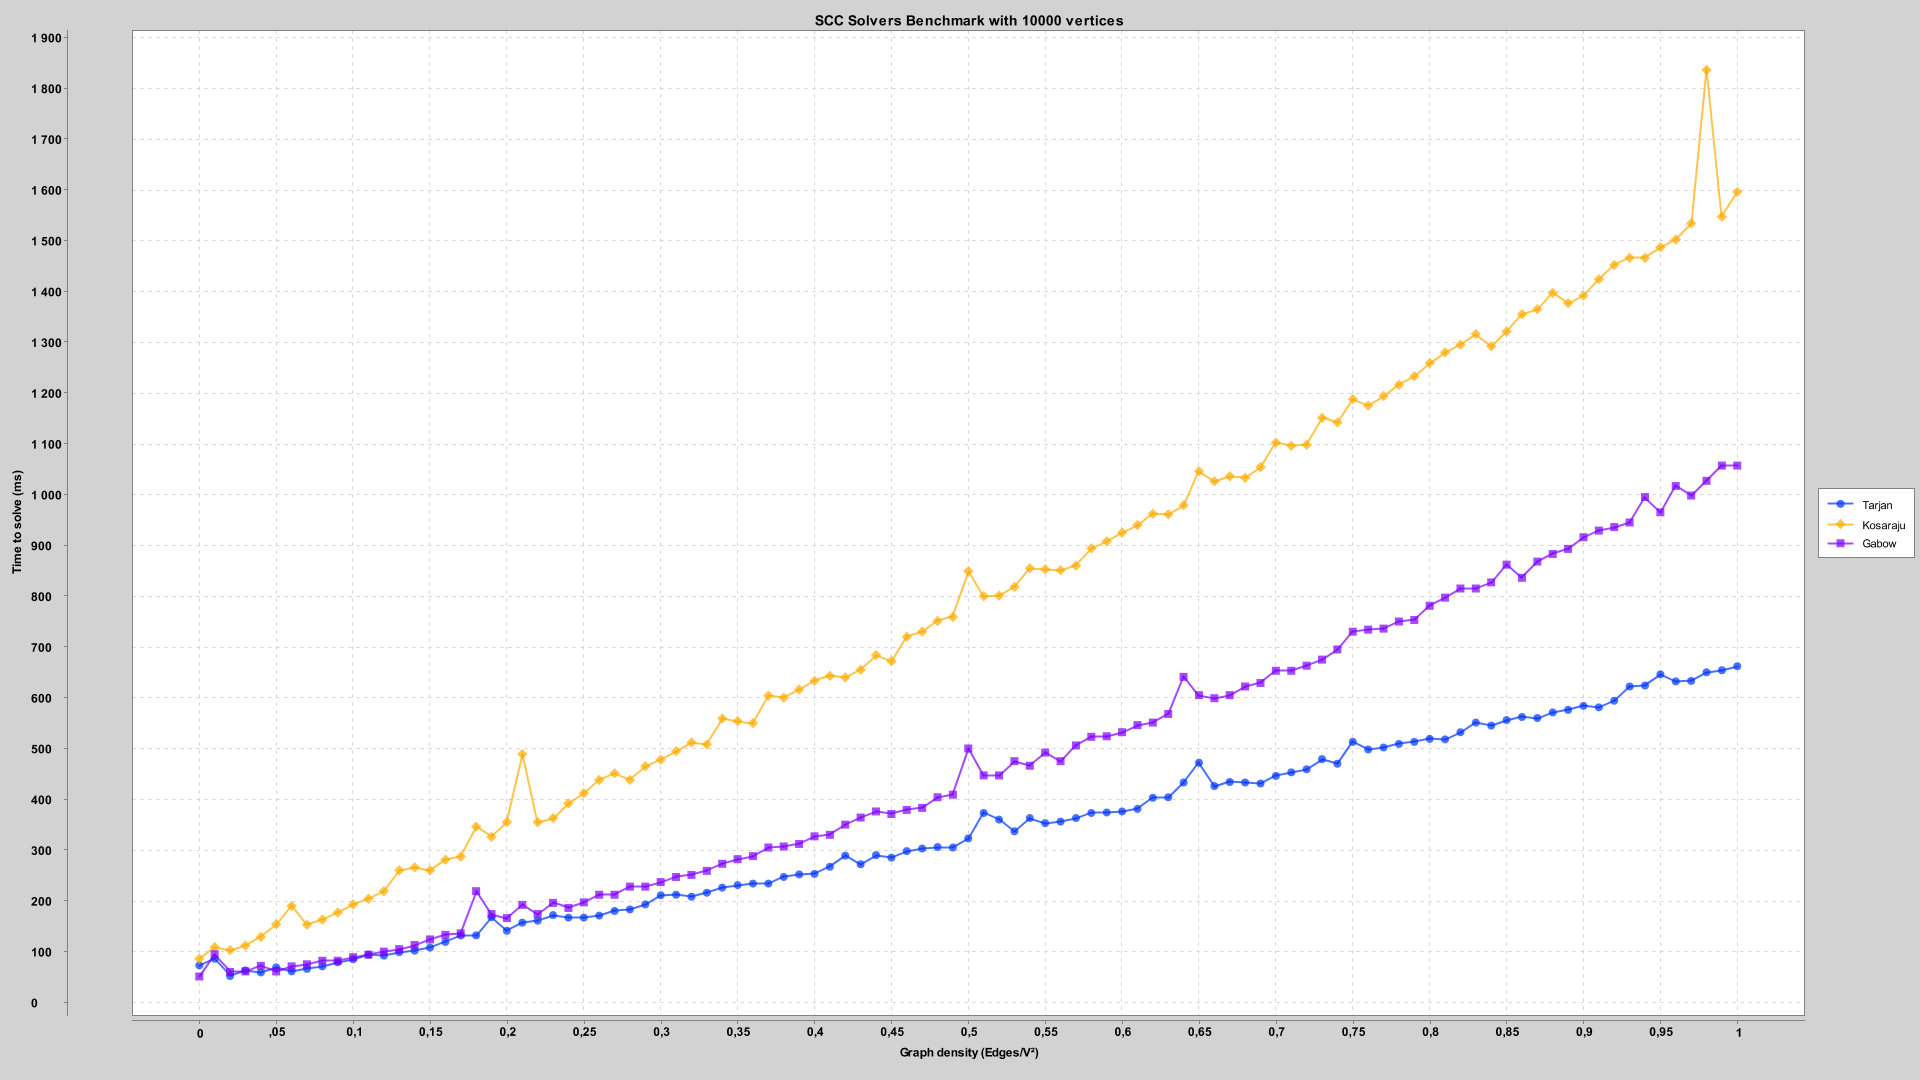
\includegraphics[keepaspectratio=true,width=\linewidth]{./SCCSolvers_10000.png}
\captionof{figure}{Évaluation de différents algorithmes de calcul de composantes fortement connexes en fonction de la densité d'un graphe à 10000 nœuds}
\end{center}

\subsubsection{V=25000}
\textbf{Soit un total de \underline{625 000 000} d'arcs lorsque la densité vaut 1.}
\begin{center}
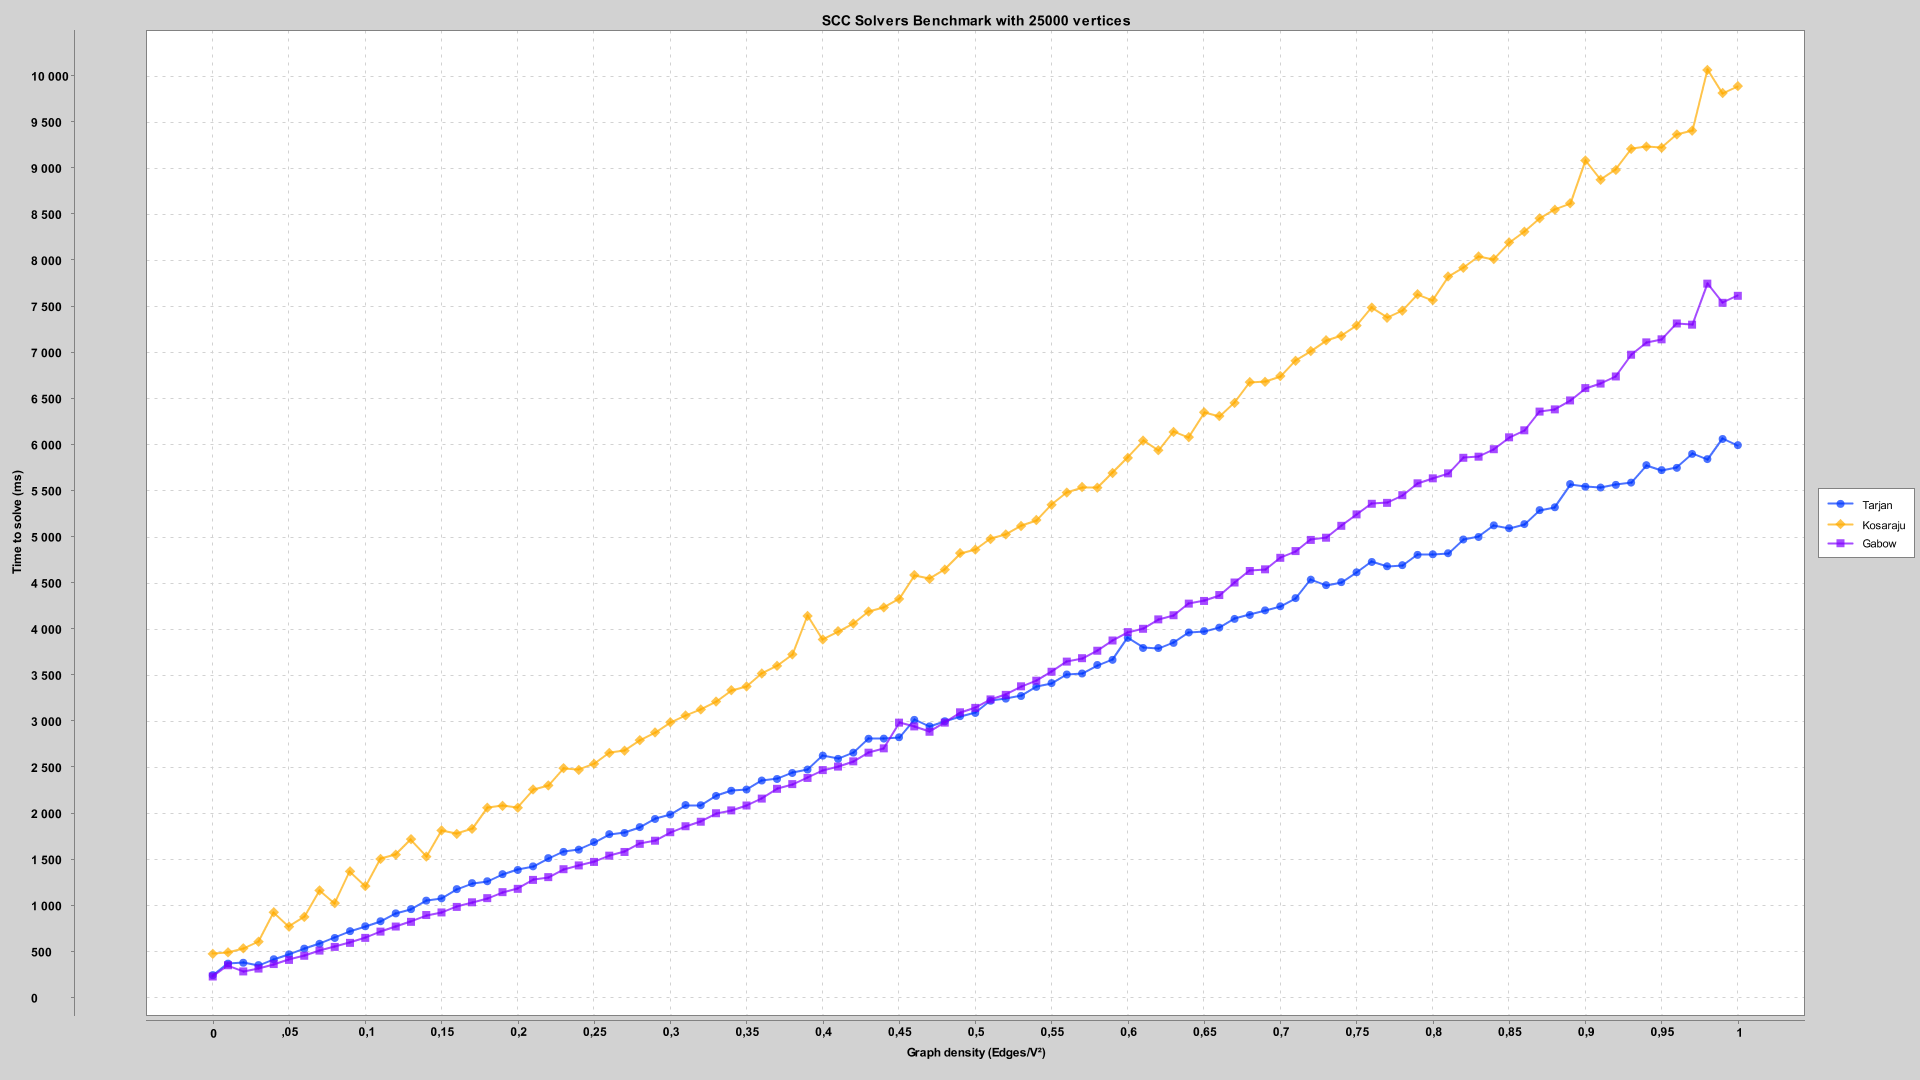
\includegraphics[keepaspectratio=true,width=\linewidth]{./SCCSolvers_25000.png}
\captionof{figure}{Évaluation de différents algorithmes de calcul de composantes fortement connexes en fonction de la densité d'un graphe à 25000 nœuds}
\end{center}

\subsection{Analyse des résultats}

Classement des algorithmes de calcul de CFC par performance :
\begin{enumerate}
\item Tarjan;
\item Gabow;
\item Kosaraju.
\end{enumerate}

Tarjan et Gabow se valent sur des graphes qui ne sont pas trop dense, après cela Tarjan est plus performant que Gabow, Kosaraju ne peut malheureusement pas entrer en concurrence avec les autres. On retiendra que les algorithmes élégants et intuitifs ne sont pas forcément les plus performants!

\end{document}
